\chapter{2026年湖北}

\begin{enumerate}
\item
%% number: 1
%% paperName: 2026年湖北高考第 1 题 4 分
%% typeId: 1
%% type: 单选题
%% chapter: 原子和原子核
%% point: 人工核反应
%% method: 无
%% score: 4
%% degree: 950
%% duplicateId: 0
%% body:
$ 2025 $ 年 $ 6 $ 月，我国成功掌握商用堆生产钇 $ 90 $（\ce{^{90}_{39} Y}）玻璃微球的技术，可实现批量化生产。在核反应堆中，\ce{^{90}_{39} Y} 由核反应 \ce{^{a}_{39} Y + ^{1}_{b} X $$ \to ^{90}_{39} Y} 生成、则 \xzanswer{D}


\fourchoices[answer=D]
{$ X $ 是质子}
{$ X $ 是电子}
{$ a =90 $}
{$ b =0 $}

%% answer: D
%% memo:
\memoanswer{
核反应遵循质量数守恒和电荷数守恒，对反应式 \ce{^{a}_{39} Y + ^{1}_{b} X $$ \to^{90}_{39} Y} 分析如下

由质量数守恒 $ a+ 1=90 $ 解得 $ a =89 $

由电荷数守恒 $ 39 +b =39 $ 解得 $ b =0 $

可知 $ X $是中子。

故选 $ D $。
}

\item
%% number: 2
%% paperName: 2026年湖北高考第 2 题 4 分
%% typeId: 1
%% type: 单选题
%% chapter: 光学
%% point: 光电效应
%% method: 无
%% score: 4
%% degree: 850
%% duplicateId: 0
%% body:
光伏产业已发展成为我国新能源三大名片之一。太阳能电池发电时，材料原子中的电子被光子激发（这也是一种光电效应），激发后的电子向电池负极移动、形成一个持续的电动势。关于太阳能电池，下列说法正确的是 \xzanswer{C} 

\fourchoices[answer=C]
{任何频率的光均可使太阳能电池发电}
{太阳光的能量可以全部转化为电池的电能}
{太阳能电池在多云的白天，仍然可以发电}
{太阳能电池发电的功率与太阳光的照射方向无关}

%% answer: C
%% memo:
\memoanswer{
已知光电效应方程为 $E_{k} = h\nu - W_{0}$，其中逸出功 $W = h\nu_{0}$，$\nu_{0}$ 为材料的极限频率。

A．只有入射光频率 $v \geq \nu_{0}$ 时，才能激发出光电子实现发电，低于极限频率的光无法产生光电效应，故 A 错误；

B．太阳能电池的光电转化效率远小于 100\%，太阳光的能量会有部分转化为内能等其他形式的能量，不可能全部转化为电能，故 B 错误；

C．多云的白天仍有频率满足要求的太阳光透过云层照射到电池板，可发生光电效应，因此仍然可以发电，故 C 正确；

D．设垂直于光传播方向的光强为 $ I_{0} $，太阳光入射方向与电池板法线的夹角为 $ \theta $，则电池板单位面积接收的光功率为 $ I = I_{0} \cos \theta $，$ \theta $不同时接收的光功率不同，发电功率也不同，因此发电功率与照射方向有关，故 D 错误。

故选 C。
}

\item
%% number: 3
%% paperName: 2026年湖北高考第 3 题 4 分
%% typeId: 1
%% type: 单选题
%% chapter: 气体性质
%% point: 理想气体状态方程
%% method: 无
%% score: 4
%% degree: 750
%% duplicateId: 0
%% body:
容器中封闭一定质量的理想气体。缓慢改变气体状态，使其体积变为初态的一半，压强变为初态的 $ 3 $ 倍。与气体的初态相比、末态 \xzanswer{B}


\fourchoices[answer=B]
{气体的温度是初态的$ 3 $倍}
{气体分子的平均动能更大}
{每个气体分子的速率都更大}
{单位时间内与容器壁单位面积碰撞的分子数更少}

%% answer: B
%% memo:
\memoanswer[shui]{
单位时间内与容器壁单位面积碰撞的分子数$\Gamma \propto \frac{P}{\sqrt{T}}$
}

\item
%% number: 4
%% paperName: 2026年湖北高考第 4 题 4 分
%% typeId: 1
%% type: 单选题
%% chapter: 电场
%% point: 带电粒子的直线运动
%% method: 无
%% score: 4
%% degree: 550
%% duplicateId: 0
%% body:
一带正电粒子仅受静电力作用，从静止开始沿直线运动，$ 0 \sim 4 t_{0} $ 时间内，其速度 $ v $ 随时间 $ t $ 的变化图像是如图所示的三条线段。$ t_{0} $ 时刻、$ 1.5 t_{0} $ 时刻、$ 3.5 t_{0} $ 时刻粒子所在位置分别为 $ a $ 点、$ b $ 点、$ c $ 点。下列说法正确的是 \xzanswer{C}


\begin{figure}[htbp]
	\centering
	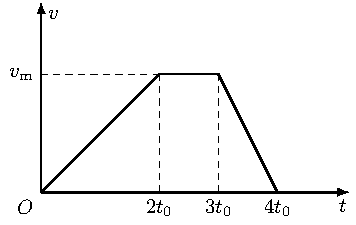
\includegraphics{tikz/2026/湖北/01.pdf}
\end{figure}

\fourchoices[answer=C]
{$b$ 点的电势比 $a$ 点的高}
{$b$ 点的电场强度比 $a$ 点的大}
{粒子在 $a$、$c$ 两点的电势能相等}
{粒子在 $a$、$c$ 两点受到的电场力大小相等}

%% answer: C

\item
%% number: 5
%% paperName: 2026年湖北高考第 5 题 4 分
%% typeId: 1
%% type: 单选题
%% chapter: 力物体的平衡
%% point: 三力平衡
%% method: 无
%% score: 4
%% degree: 550
%% duplicateId: 0
%% body:
如图所示，半径为 $ R $ 的光滑圆环固定在竖直平面内，原长为 $ 2 \sqrt 3 R $ 的轻质弹簧一端固定在圆环上与圆心 $ O $ 等高的位置，另一端连接一个套在圆环上质量为 $ m $ 的小球，平衡时弹簧与水平方向的夹角为 $ 30 {^\circ} $。弹簧在弹性限度内，重力加速度大小为 $ g $，弹簧的劲度系数为 \xzanswer{C}
\begin{figure}[htbp]
	\centering
	\includesvg[width=127.5pt,height=127.5pt]{pic/2026/湖北/02}
\end{figure}

\fourchoices[answer=C]
{$ \frac{{\sqrt 3 mg}}{{6R}} $}
{$ \frac{{mg}}{{2R}} $}
{$ \frac{{\sqrt 3 mg}}{{3R}} $}
{$ \frac{{mg}}{R} $}

%% answer: C

\item
%% number: 6
%% paperName: 2026年湖北高考第 6 题 4 分
%% typeId: 1
%% type: 单选题
%% chapter: 曲线运动
%% point: 开普勒定律
%% method: 无
%% score: 4
%% degree: 450
%% duplicateId: 0
%% body:
已知某卫星绕地球做椭圆运动，在近地点所受的地球引力为其在地面附近的 $ \frac{1}{4} $，在远地点所受的地球引力为其在地面附近的 $ \frac{1}{16} $。地面附近的重力加速度大小为 $ g $，地球半径为 $ R $，该卫星的运动周期为 \xzanswer{B}


\fourchoices[answer=B]
{$ 4 \pi\sqrt {\frac{{2R}}{g}} $}
{$ 6 \pi\sqrt {\frac{{3R}}{g}} $}
{$ 16 \pi\sqrt {\frac{{R}}{g}} $}
{$ 12 \pi\sqrt {\frac{{6R}}{g}} $}

%% answer: B

\item
%% number: 7
%% paperName: 2026年湖北高考第 7 题 4 分
%% typeId: 1
%% type: 单选题
%% chapter: 电磁感应
%% point: 电磁感应与动量定理
%% method: 无
%% score: 4
%% degree: 450
%% duplicateId: 0
%% body:
如图所示，固定在水平面内的两足够长平行金属导轨相距 $ L $，其左端用导线连接一阻值为 $ R $ 的电阻，两导轨间存在垂直于导轨平面向下的匀强磁场，磁感应强度大小为 $ B $。质量为 $ m $ 的导体棒跨放在两导轨上，导体棒在两导轨间的电阻为 $ 2 R $。导轨上 $ a $、$ b $、$ c $、$ d $ 是正方形的四个顶点。导体棒以大小为 $ \frac{{4{B^2}{L^3}}}{{mR}} $ 的初速度从 $ ab $ 出发沿导轨向右运动，刚过 $ cd $ 后，$ abcd $ 区域内磁场的磁感应强度方向不变、大小在极短时间内增大到 $ 3 B $，然后保持不变。导体棒运动过程中始终与导轨垂直，且与导轨接触良好，不计导轨电阻与所有摩擦，导体棒最终静止的位置离初始位置的距离为 \xzanswer{B}
\begin{figure}[htbp]
	\centering
	\includesvg[width=165.0pt,height=99.0pt]{pic/2026/湖北/03}
\end{figure}

\fourchoices[answer=B]
{$ 9 L $}
{$ 10 L $}
{$ 11 L $}
{$ 12 L $}

%% answer: B

\item
%% number: 8
%% paperName: 2026年湖北高考第 8 题 4 分
%% typeId: 2
%% type: 多选题
%% chapter: 交流电
%% point: 变压器
%% method: 无
%% score: 4
%% degree: 550
%% duplicateId: 0
%% body:
如图所示，有一理想变压器，其原线圈输入电压为 $ u =100 \sqrt 2 \sin 100 \pi t \UV $，在一个副线圈上接额定电压为 $ 220 \UV $、额定功率为 $ 10 \UW $ 的灯泡甲，在另一个单匝副线圈上接额定电压为 $ 2 \UV $、额定功率为 $ 1 \UW $ 的灯泡乙，两灯泡均能正常发光。下列说法正确的是 \xzanswer{AC}
\begin{figure}[htbp]
	\centering
	\includesvg[width=210.0pt,height=98.2pt]{pic/2026/湖北/04}
\end{figure}

\fourchoices[answer=AC]
{原线圈的匝数为 $ 50 $}
{输入电压的频率为 $ 100 \UHz $}
{原线圈的输入功率为 $ 11 \UW $}
{流过原线圈的电流最大值为 $ 0.11 \UA $}

%% answer: AC

\item
%% number: 9
%% paperName: 2026年湖北高考第 9 题 4 分
%% typeId: 2
%% type: 多选题
%% chapter: 曲线运动
%% point: 竖直平面圆周运动
%% method: 无
%% score: 4
%% degree: 350
%% duplicateId: 0
%% body:
如图所示，半径为 $ R $、内壁光滑的圆环轨道固定在竖直平面内。初始时刻，质量为 $ m $ 的小球甲从圆环内表面最高处以大小为 $ v_{0} = \sqrt {2gR} $（$ g $为重力加速度大小）的水平初速度向右运动，同时质量为 $ 2 m $ 的小球乙从圆环内表面最低处以某一水平初速度向左运动。当甲第一次运动到圆环最低点时，乙恰好第一次运动到圆环最高点。不计空气阻力，下列说法正确的是 \xzanswer{BD}
\begin{figure}[htbp]
	\centering
	\includesvg[width=127.5pt,height=174.0pt]{pic/2026/湖北/05}
\end{figure}

\fourchoices[answer=BD]
{乙的初速度大小为 $ 3 \sqrt {gR} $}
{甲、乙两小球运动的周期相等}
{任意时刻两小球的连线均过圆环圆心}
{任意时刻两小球对圆环作用力的合力均不为零}

%% answer: BD
%% memo:
\memoanswer[shui]{
	首先要证明在圆轨道上运动的时间与质量无关。
	
	以最高点为参考点，与圆心连线转过的角度为$\theta$，角度速为$\omega^{2} R=2g-3g\cos\theta+\frac{v_0}{R}$，角速度与质量无关，运动时间也与质量无关。
}

\item
%% number: 10
%% paperName: 2026年湖北高考第 10 题 4 分
%% typeId: 2
%% type: 多选题
%% chapter: 曲线运动
%% point: 斜抛运动
%% method: 极值
%% score: 4
%% degree: 350
%% duplicateId: 0
%% body:
某山沟竖直截面图如图所示，山沟的一侧竖直，另一侧是以 $ O $ 点为圆心、$ R $ 为半径的 $ \frac{1}{4} $ 圆弧，圆弧最高点与 $ O $ 点等高。救援队从 $ O $ 点以大小为 $ v_{0} = \frac{{\sqrt {2gR} }}{2} $ 的初速度向该山沟投掷救援物资，其中 $ g $ 是重力加速度大小。物资可视为质点，不计空气阻力。为避免损坏救援物资，要求物资落到圆弧上的速率最小，则物资 \xzanswer{AD}
\begin{figure}[htbp]
	\centering
	\includesvg[width=112.5pt,height=107.2pt]{pic/2026/湖北/06}
\end{figure}

\fourchoices[answer=AD]
{在空中运动的时间为 $ \sqrt {\frac{{2R}}{g}} $}
{与水平方向成 $ 45 {^\circ} $ 角斜上抛}
{抛出点与落点的高度差为 $ \frac{{\sqrt 2 R}}{2} $}
{落到圆弧上的最小速率为 $ \frac{{\sqrt {6gR} }}{2} $}

%% answer: AD
%% memo:
\memoanswer[shui]{
	可以用函数法，但计算较为繁琐。当高度、初速度大小一定时，以什么角度抛物体抛得最远，最远距离是多少，这些相关结论，也可用于此题的求解。
}

\item
%% number: 11
%% paperName: 2026年湖北高考第 11 题 8 分
%% typeId: 4
%% type: 实验题
%% chapter: 电路
%% point: 测量电阻率
%% method: 无
%% score: 8
%% degree: 550
%% duplicateId: 0
%% body:
在测量铅笔芯电阻率的实验中，实验器材有：待测圆柱形铅笔芯、电压表 $ \mathrm{V} $、电流表 $ \mathrm{A} $、电阻箱 $ R_{0} $、干电池、刻度尺、螺旋测微器、开关 $ S $、滑片 $ P $ 及导线等。实验电路图如图~\subref{2026湖北07} 所示，$ B $、$ C $ 为铅笔芯的两端，滑片 $ P $ 在 $ B $、$ C $ 间左右滑动。
\begin{figure}[htbp]
\centering
\begin{subfigure}{0.48\linewidth}
	\centering
	\includesvg[width=195.0pt,height=159.8pt]{pic/2026/湖北/07}
	\caption{}\label{2026湖北07}
\end{subfigure}
\hfil
\begin{subfigure}{0.33\linewidth}
	\centering
	\includesvg[width=97.5pt,height=151.5pt]{pic/2026/湖北/08}
	\caption{}\label{2026湖北08}
\end{subfigure}
\end{figure}
\begin{enumerate}
\item
用螺旋测微器测量铅笔芯的直径 $d$，其示数如图~\subref{2026湖北08} 所示，可知 $d=$ \tkanswer{$0.500$} $\Umm[a]$。
\item
适当选择电阻箱 $ R_{0} $ 的阻值、移动滑片 $ P $ 到某位置、测量 $ B $、$ P $ 间的长度 $ L $，闭合开关 $ S $，记录电压表的示数 $ U $，电流表的示数 $ I $，则该铅笔芯电阻率的表达式为 $ \rho = $ \tkanswer{$\frac{{\pi U{d^2}}}{{4IL}}$}（用 $ U $、$ I $、$ d $ 和 $ L $ 表示）。
\item
多次改变滑片 $ P $ 的位置、记录对应的 $ L $、$ U $、$ I $，由实验数据绘制出的 $ U-IL $ 图如图~\subref{2026湖北09} 所示。由此可得该铅笔芯的电阻率 $ \rho = $ \tkanswer{$6.4\times10^{-6}$} $ \UOm[a] $（$ \pi $ 取 $ 3.14 $，保留两位有效数字）。
\begin{figure}[htbp]
	\centering
	\begin{subfigure}{0.65\linewidth}
		\centering
		\setcounter{subfigure}{2}
		\includesvg[width=315.0pt,height=229.5pt]{pic/2026/湖北/09}
		\caption{}\label{2026湖北09}
	\end{subfigure}
\end{figure}
\item
干电池使用一段时间后，其内阻增大，对电阻率的测量结果\tkanswer{无}（填“有”或“无”）影响。	
\end{enumerate}


%% answer:
\jdanswer{
\begin{enumerate}
	\item 
	$0.500$
	
	\item
	$\frac{{\pi U{d^2}}}{{4IL}}$
	
	\item
	$6.4\times10^{-6}$
	
	\item
	无
\end{enumerate}
}

\item
%% number: 12
%% paperName: 2026年湖北高考第 12 题 9 分
%% typeId: 4
%% type: 实验题
%% chapter: 运动和力
%% point: 验证牛顿第二定律
%% method: 无
%% score: 9
%% degree: 450
%% duplicateId: 0
%% body:
某同学设计了一个验证牛顿第二定律的实验，使用的器材有：直导轨、小车、光电门、数字毫秒计、遮光条、天平、钩码、刻度尺、游标卡尺、定滑轮、细绳等。实验装置如图所示，光电门 $ 1 $、$ 2 $ 分别固定在导轨 $ A $、$ B $ 处，遮光条安装在小车上，连接小车两端的细绳分别跨过左右定滑轮、各悬挂 $ 10 $ 个质量均为 $ m_{0} $ 的钩码，定滑轮间的细绳与导轨平行。重力加速度大小为 $ g $。实验步骤如下：
\begin{figure}[htbp]
\centering
\includesvg[width=375.0pt,height=168.8pt]{pic/2026/湖北/10}
\end{figure}
\begin{enumerate}[label=\roman*.]
	\item 
	用天平测量小车和遮光条的总质量 $ m $，用刻度尺测量 $ A $、$ B $ 间的距离 $ s $，用游标卡尺测量遮光条的宽度 $ d $。
	\item 
	调节导轨倾斜程度，使小车沿导轨向右下滑时通过两个光电门的遮光时间近似相等。
	\item 
	从左侧细绳取下 $ n $ 个钩码挂到右侧细绳，再从导轨左端静止释放小车，用数字毫秒计测量遮光条经过光电门 $ 1 $、$ 2 $ 的遮光时间 $ t_{1} $、$ t_{2} $。
\end{enumerate}
回答下列问题：
\begin{enumerate}
	\item 
	步骤 \ronum{2} 操作的主要目的是\tkanswer{平衡摩擦力}。
	
	\item
	由牛顿第二定律，小车的加速度大小 $ a =$\tkanswer{$\frac{{2n{m_0}g}}{{m + 20{m_0}}}$}（用 $ m_{0} $、$ m $、$ g $ 和 $ n $ 表示）。
	
	\item
	步骤 \ronum{3} 中测得的小车加速度大小 $ a =$\tkanswer{$\frac{{{d^2}}}{{2s}}\left( {\frac{1}{{t_2^2}} - \frac{1}{{t_1^2}}} \right)$}（用 $ d $、$ s $、$ t_{1} $ 和 $ t_{2} $ 表示）。
	
	\item
	该同学根据测出的多组 $ a $、$ n $ 值，作出 $ a-n $ 图像。若该图像近似是一条通过原点的直线，则可以验证：质量一定时，物体的加速度与所受合外力成\tkanswer{正比}。
	
	\item
	若 $ a-n $ 图像明显不过原点，原因可能是\tkanswer{B}（单选，填标号）。
	\threechoices[answer=B]
	{步骤 \ronum{3} 中小车没有从静止释放}
	{步骤 \ronum{2} 中导轨的倾斜程度调节不恰当}
	{钩码质量没有远小于小车和遮光条的总质量}
	
\end{enumerate}


%% answer:
\jdanswer{
\begin{enumerate}
	\item 
	平衡摩擦力
	
	\item
	$\frac{{2n{m_0}g}}{{m + 20{m_0}}}$
	
	\item
	$\frac{{{d^2}}}{{2s}}\left( {\frac{1}{{t_2^2}} - \frac{1}{{t_1^2}}} \right)$
	
	\item
	正比
	
	\item
	B
\end{enumerate}
}

\item
%% number: 13
%% paperName: 2026年湖北高考第 13 题 9 分
%% typeId: 6
%% type: 计算题
%% chapter: 机械波
%% point: 波的图象
%% method: 无
%% score: 9
%% degree: 550
%% duplicateId: 0
%% body:
一列简谐横波沿 $ x $ 轴传播，波速为 $ v =2 \Ums $。$ t =0 $ 时刻的波形图如图所示，此时 $ x =3\Um $ 处的质点$ P $的振动方向沿 $ y $ 轴负方向，$ x =5 \Um $ 和 $ x =11 \Um $ 处的质点均处于平衡位置。
\begin{enumerate}
	\item 
	求波的传播方向、波长 $ \lambda $ 和周期 $ T $。
	
	\item
	从 $ t =0 $ 时刻开始，经多长时间质点 $ P $ 第二次到达平衡位置？
\end{enumerate}
\begin{figure}[htbp]
	\raggedleft
	\includesvg[width=240.0pt,height=125.2pt]{pic/2026/湖北/11}
\end{figure}
%% answer:
\jdanswer{
\begin{enumerate}
	\item 
	沿 $ x $ 负方向传播，$ \lambda =12 \Um $，$ T =6 \Us $
	
	\item
	$ 4 \Us $
\end{enumerate}
}

\item
%% number: 14
%% paperName: 2026年湖北高考第 14 题 16 分
%% typeId: 6
%% type: 计算题
%% chapter: 磁场
%% point: 带电粒子在组合场中的运动
%% method: 无
%% score: 16
%% degree: 450
%% duplicateId: 0
%% body:
如图所示，在 $ xOy $ 平面内，$ y >0 $ 区域存在匀强电场，电场强度大小为 $ E $、方向沿 $ y $ 轴负方向；在 $ y <0 $ 区域，有一个以 $ O $ 为圆心、$ r $ 为半径的半圆形区域，半圆形区域内既无电场也无磁场，半圆形区域外存在匀强磁场，磁场方向垂直于 $ xOy $ 平面向里。一质量为 $ m $、电荷量为 $ q $ 的带正电粒子从坐标为$( 0 , \frac{{25}}{{12}}r )$的 $ M $ 点静止释放，之后从坐标为$( 2r,0 )$的 $ N $ 点第一次射出磁场。不计重力，求：
\begin{enumerate}
	\item 
	粒子第一次进入磁场时的速度大小；
	
	\item
	磁场的磁感应强度大小；
	
	\item
	粒子第二次射出磁场时的位置坐标。
\end{enumerate}
\begin{figure}[htbp]
	\raggedleft
	\includesvg[width=202.5pt,height=219.0pt]{pic/2026/湖北/12}
\end{figure}
%% answer:
\jdanswer{
\begin{enumerate}
	\item 
	$ \sqrt {\frac{{25qEr}}{{6m}}} $
	
	\item
	$ \sqrt {\frac{{8mE}}{{3qr}}} $
	
	\item
	$(0,-r) $
\end{enumerate}
}
%% memo:
\memoanswer[shui]{
	半圆顶点与$N$连线与$x$轴夹角为$\theta$，粒子第一次出磁场时与$x$轴的夹角$\sin2\theta= \frac{4}{5} $，画出第二次进入磁场的轨迹图，其与$y$轴相切，切点刚好是半圆顶点。
}


\item
%% number: 15
%% paperName: 2026年湖北高考第 15 题 18 分
%% typeId: 6
%% type: 计算题
%% chapter: 运动和力
%% point: 动量和能量
%% method: 分情况讨论
%% score: 18
%% degree: 350
%% duplicateId: 0
%% body:
在如图所示的竖直平面内，固定在水平地面上的光滑轨道由两倾角均为 $ 30 {^\circ} $ 的足够长轨道与一水平轨道平滑连接而成，连接点分别为 $ A $、$ B $。质量为 $ m $ 的小物块甲放置在左侧倾斜轨道上高 $ h $ 处、质量为 $ km $ 的小物块乙静止在水平轨道上，乙到 $ A $、$ B $ 两点的距离均为 $ h $。现静止释放甲，所有碰撞均为弹性正碰，重力加速度大小为 $ g $，不计空气阻力。
\begin{enumerate}
	\item 
	求甲第一次到达 $ A $ 点时的速度大小。
	
	\item
	求两物块第一次碰撞过程中，乙所受合外力的冲量大小。
	
	\item
	若两物块在水平轨道上发生第二次碰撞，且第二次碰撞前只有一个物块滑上倾斜轨道，求 $ k $ 满足的关系式（不求具体数值）。
\end{enumerate}
\begin{figure}[htbp]
	\raggedleft
	\includesvg[width=430.0pt,height=114.0pt]{pic/2026/湖北/13}
\end{figure}
%% answer:
\jdanswer{
\begin{enumerate}
	\item 
	$ v_{0} = \sqrt {2gh} $
	
	\item
	$ I = \frac{2km}{{1 + k}}\sqrt{2gh} $
	
	\item
	$ 0.81 \leq k \leq 1.2 $ 或 $ k \geq 20.1 $
\end{enumerate}
}
%% memo:
\memoanswer[shui]{
	第三问计算较为繁琐，需要讨论几种情况。
	
	$k=1$显然成立。
	
	甲乙同向时，$k<1$，有$\frac{2}{1-k}-\frac{32}{(1+k)^2}>1$，虽然有解析解，但表达式复杂，数值解为$k>0.8136$。
	
	甲乙反向时，需要讨论甲乙谁跑得快，即$1<k<3$和$k>3$，再立不等式方程即可求解。
}

\end{enumerate}
